\documentclass{article}

% if you need to pass options to natbib, use, e.g.:
\PassOptionsToPackage{numbers, compress}{natbib}
% before loading neurips_2026

% The authors should use one of these tracks.
% Before accepting by the NeurIPS conference, select one of the options below.
% 0. "default" for submission
\usepackage{neurips_2026}


% After being accepted, the authors should add "final" behind the track to compile a camera-ready version.
% 1. Main Track
 % \usepackage[main, final]{neurips_2026}
% 2. Position Paper Track
%  \usepackage[position, final]{neurips_2026}
% 3. Evaluations & Datasets Track
 % \usepackage[eandd, final]{neurips_2026}
% 4. Creative AI Track
%  \usepackage[creativeai, final]{neurips_2026}
% 5. Workshop with single-blind reviewing
%  \usepackage[sglblindworkshop, final]{neurips_2026}
% 6. Workshop with double-blind reviewing
%  \usepackage[dblblindworkshop, final]{neurips_2026}
% Note. For the workshop paper template, both \title{} and \workshoptitle{} are required, with the former indicating the paper title shown in the title and the latter indicating the workshop title displayed in the footnote.
% For workshops (5., 6.), the authors should add the name of the workshop, "\workshoptitle" command is used to set the workshop title.
% \workshoptitle{WORKSHOP TITLE}

% "preprint" option is used for arXiv or other preprint submissions
 % \usepackage[preprint]{neurips_2026}

% to avoid loading the natbib package, add option nonatbib:
%    \usepackage[nonatbib]{neurips_2026}

\usepackage[utf8]{inputenc} % allow utf-8 input
\usepackage[T1]{fontenc}    % use 8-bit T1 fonts
\usepackage{hyperref}       % hyperlinks
\usepackage{url}            % simple URL typesetting
\usepackage{booktabs}       % professional-quality tables
\usepackage{amsfonts}       % blackboard math symbols
\usepackage{nicefrac}       % compact symbols for 1/2, etc.
\usepackage{microtype}      % microtypography
\usepackage{xcolor}         % colors
\usepackage{amsmath}
\usepackage{wrapfig}
\usepackage{enumitem}


\definecolor{tabblue}{HTML}{1F77B4}
\definecolor{taborange}{HTML}{FF7F0E}
\definecolor{tabgreen}{HTML}{2CA02C}
\definecolor{tabred}{HTML}{D62728}
\definecolor{tabpurple}{HTML}{9467BD}
\definecolor{tabbrown}{HTML}{8C564B}
\definecolor{tabpink}{HTML}{E377C2}
\definecolor{tabgray}{HTML}{7F7F7F}
\definecolor{tabolive}{HTML}{BCBD22}
\definecolor{tabcyan}{HTML}{17BECF}

\usepackage{rotating} 
\usepackage[most]{tcolorbox}
\newtcolorbox{takeaway}{
  colback=blue!5,
  colframe=blue!5,
  width=1\textwidth,
  boxrule=0pt,
  left=5pt, right=5pt, top=3pt, bottom=3pt, % Halved padding
  boxsep=0pt, % Removes default invisible boundary space
  %fontupper=\small % Scales down from \normalsize
}


\title{Cornerstones or Stumbling Blocks? Deciphering the Rock Tokens in On-Policy Distillation}


% The \author macro works with any number of authors. There are two commands
% used to separate the names and addresses of multiple authors: \And and \AND.
%
% Using \And between authors leaves it to LaTeX to determine where to break the
% lines. Using \AND forces a line break at that point. So, if LaTeX puts 3 of 4
% authors names on the first line, and the last on the second line, try using
% \AND instead of \And before the third author name.


\author{
Yuxuan Jiang$^{1,*}$,
Runchao Li$^{2,*}$,
Shubhashis Roy Dipta$^{1,*}$,
Dawei Li$^{3}$,
Zhao Yang$^{4,\dagger}$\\
$^{1}$UMBC \quad
$^{2}$Case Western Reserve University \quad
$^{3}$Arizona State University \quad
$^{4}$VU Amsterdam\\
$^{*}$Equal contribution \quad
$^{\dagger}$Corresponding author
}


\begin{document}


\maketitle


\begin{abstract}


% On-Policy Distillation (OPD) has emerged as a pivotal technique in the post-training of Large Language Models (LLMs), achieving precise and efficient alignment by providing token-level supervision on student-generated trajectories. Previous studies have shown that high-loss tokens are regarded as critical correction points where the student significantly deviates from the teacher, thereby driving the learning process. This view assumes that high-loss tokens should vanish with sufficient training; however, our empirical analysis shows otherwise. Even after OPD training reaches apparent saturation, a substantial subset of tokens continues to exhibit persistently high loss; these tokens, which we term \textbf{Rock Tokens}, can account for up to 50\% of the tokens in generated outputs. Our investigation reveals two startling paradoxes. First, despite their high occurrence frequency providing a disproportionately large share of total gradient norms, Rock Tokens themselves remain \textit{stagnant} throughout training, resisting teacher-driven corrections. Second, through causal intervention, we find that these tokens provide negligible functional contribution to the model's actual reasoning performance. These findings suggest that a vast amount of optimization bandwidth is spent on structural and discourse residuals that the student model cannot or need not internalize. By deconstructing these dynamics, we demonstrate that strategically bypassing these ``stumbling blocks'' can significantly streamline the alignment process, challenging the necessity of uniform token weighting and offering a more efficient paradigm for large-scale model distillation.

While recent work in Reinforcement Learning with Verifiable Rewards (RLVR) has shown that a small subset of critical tokens disproportionately drives reasoning gains, an analogous token-level understanding of On-Policy Distillation (OPD) remains largely unexplored. In this work, we investigate high-loss tokens, a token type that—as the most direct signal of student-teacher mismatch under OPD's per-token KL objective—should progressively diminish as training converges according to existing studies; however, our empirical analysis shows otherwise. Even after OPD training reaches apparent saturation, a substantial subset of tokens continues to exhibit persistently high loss; these tokens, which we term Rock Tokens, can account for up to 50\% of the tokens in generated outputs. Our investigation reveals two startling paradoxes. First, despite their high occurrence frequency providing a disproportionately large share of total gradient norms, Rock Tokens themselves remain stagnant throughout training, resisting teacher-driven corrections. Second, through causal intervention, we find that these tokens provide negligible functional contribution to the model's actual reasoning performance. These findings suggest that a vast amount of optimization bandwidth is spent on structural and discourse residuals that the student model cannot or need not internalize. By deconstructing these dynamics, we demonstrate that strategically bypassing these "stumbling blocks" can significantly streamline the alignment process, challenging the necessity of uniform token weighting and offering a more efficient paradigm for large-scale model distillation.
\end{abstract}






\section{Introduction}

On-Policy Distillation (OPD) has established itself as a cornerstone of the modern post-training pipeline for Large Language Models (LLMs). By aligning a student model with a superior teacher through trajectories sampled from its own policy, OPD enables a token level of reasoning refinement that goes beyond static Supervised Fine-Tuning (SFT). This effectiveness has been validated by industrial works such as DeepSeek-V4~\cite{deepseekv4}, MiMo~\cite{xiao2026mimo}, and Qwen-3~\cite{qwen3technicalreport}, where OPD serves as a vital component alongside SFT or Reinforcement Learning with Verifiable Rewards (RLVR) to further squeeze out reasoning performance.


% In existing OPD research, high-loss tokens are generally characterized as potential "critical branching points" where the student's policy deviates significantly from the teacher's trajectory, thus serving as the primary drivers of policy correction~\cite{lu2025onpolicydistillation}. Intuitively, as the student aligns with the teacher during the OPD process, both the magnitude and cardinality of these high-loss tokens are expected to diminish, eventually leading to an optimization plateau. However, our empirical investigations reveal a striking phenomenon: even after training has reached apparent saturation, a stubborn population of tokens—which we formally define as \textbf{Rock Tokens}—continues to exhibit consistently high loss. Notably, while these tokens represent a small minority of the vocabulary (approximately 6\%), they account for as much as 50\% of the total token frequency in the model's output. This persistence challenges conventional understanding of model convergence and raises a fundamental question: \textit{Are Rock Tokens indispensable Pillars for policy alignment, or are they Stumbling Blocks that create unnecessary optimization redundancy?}

Recent studies in Reinforcement Learning with Verifiable Rewards (RLVR) have revealed that not all tokens contribute equally to model learning: a small subset of critical tokens, such as high-entropy "forking tokens" at decisive branching points, disproportionately drives reasoning gains~\cite{wang2025beyond}. While this token-level perspective has reshaped our understanding of RLVR dynamics, an analogous investigation in OPD remains largely unexplored, despite OPD's reliance on dense token-level supervision. In this work, we initiate such an investigation by focusing on a token type uniquely meaningful to the OPD paradigm: high-loss tokens. Unlike RLVR, where token importance is inferred from policy entropy or reward signals, OPD provides a direct measure of student-teacher mismatch through per-token KL divergence; high-loss tokens thus explicitly mark the positions where the student's policy diverges most sharply from the teacher's, making them natural candidates for the ``critical correction points'' that drive alignment~\cite{lu2025onpolicydistillation}. 

Intuitively, as the student aligns with the teacher during the OPD process, both the magnitude and cardinality of these high-loss tokens are expected to diminish, eventually leading to an optimization plateau. However, our empirical investigations reveal a striking phenomenon: even after training has reached apparent saturation, a stubborn population of tokens—which we formally define as Rock Tokens—continues to exhibit consistently high loss. Notably, while these tokens represent a small minority of the vocabulary (approximately 6\%), they account for as much as 50\% of the total token frequency in the model's output. This persistence challenges conventional understanding of model convergence and raises a fundamental question: Are Rock Tokens indispensable Pillars for policy alignment, or are they Stumbling Blocks that create unnecessary optimization redundancy?


\begin{figure}[t]
  \centering
  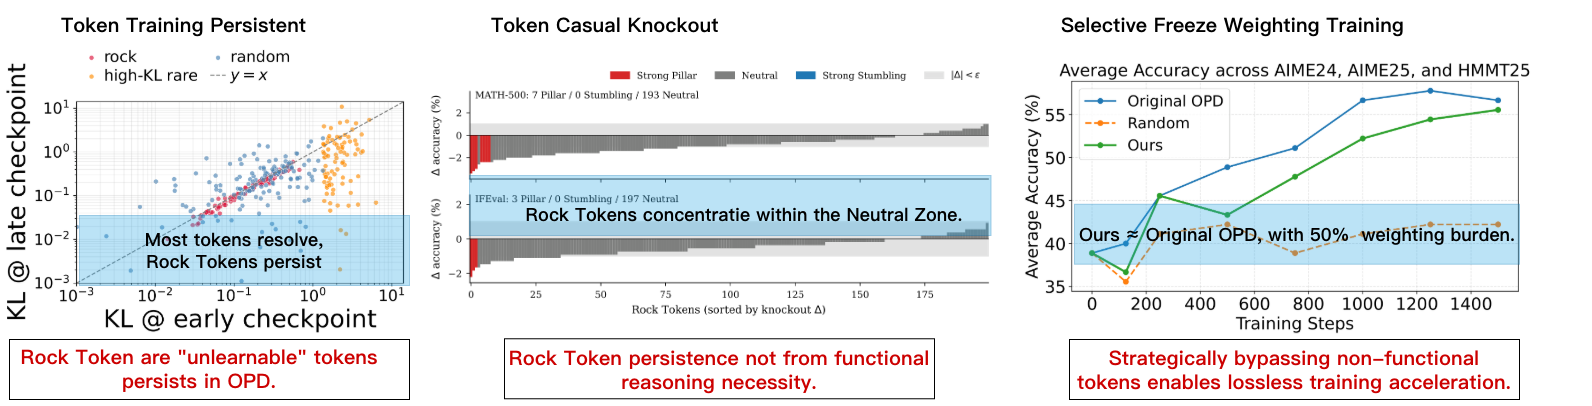
\includegraphics[width=\linewidth]{Figures/rock_intro.png}
  \caption{\textbf{The lifecycle and functional impact of Rock Tokens in OPD.} (a) \textbf{Phenomenon}: Identification of optimization-resistant tokens. (b) \textbf{Mechanism}: Causal evidence of structural redundancy via token knock-out. (c) \textbf{Utility}: Performance parity achieved through strategic gradient sparsification.}
  \label{fig:intro}
\end{figure}



To provide a systematic understanding of the Rock Token phenomenon, our research is structured across three investigative dimensions: identifying \textbf{what} are rock tokens, analyzing \textbf{why} they emerge and persist, and uncovering \textbf{how} they collectively impact the overall OPD training process. This comprehensive framework is operationalized through the following three stages:

First, we characterize the identity of Rock Tokens (What). We begin by identifying Rock Tokens linguistic and statistical properties, revealing that they primarily comprise \textbf{syntactic and structural scaffolding}—such as formatting delimiters, whitespace symbols, and high-frequency discourse markers (e.g., ``So'', ``Wait''). To determine the dynamic role of these elements, we employ quantitative gradient dynamics analysis to address \textbf{RQ1: Do Rock Tokens still provide useful learning signals during optimization?} By examining whether their persistent high loss effectively translates into constructive gradients, we assess whether these tokens offer steady directional guidance or merely represent stagnant optimization noise throughout the OPD process.

Second, we investigate the underlying mechanisms behind their persistence (Why). Beyond the actual contribution of Rock Tokens during training is clarified, a more profound question emerges: \textbf{why do these tokens persist in the first place?} We hypothesize that the student model develops a strong decoding dependency on these specific tokens to maintain its reasoning flow, creating a path dependency that resists corrections from the teacher model. This leads to our \textbf{RQ2: Does Rock Token persistence stem from student path dependency?} To investigate this, we conduct \textit{token knock-out} experiments as a form of ablation analysis, examining whether the student's logical coherence is so deeply intertwined with these persistent residuals that it becomes structurally unable to shift its policy toward the teacher's distribution.

Finally, we evaluate how Rock Tokens influence the overall OPD training process (How). Finally, we arrive at a provocative question: what would happen if these tokens were excluded from the very beginning of OPD training? This leads to our final investigation, \textbf{RQ3: What is the genuine functional contribution of Rock Tokens to model training?} By freezing the gradients of these tokens from the onset of training, we intuitively isolate their functional necessity throughout the entire distillation process. This causal intervention allows us to rigorously determine whether Rock Tokens serve as indispensable pillars of the model's reasoning integrity or if they represent a strategic opportunity to bypass computational redundancy and optimize the efficiency of the alignment pipeline.

In summary, our key contributions are as follows:


\begin{itemize}[leftmargin=*,itemsep=1pt]
    \vspace{-2mm}
    \item For the first time, we identify and characterize \textbf{Rock Tokens}, a persistent high-loss phenomenon that unveils a previously hidden aspect of optimization dynamics in On-Policy Distillation.
    \vspace{-1mm}
    \item We deconstruct the intricate dynamics of the OPD process by systematically uncovering the functional roles of Rock Tokens across both the training and inference phases.
    \vspace{-1mm}
    \item Our research reveals a critical inefficiency in current alignment pipelines, demonstrating that a substantial portion of training signals in OPD provides significantly lower-than-expected contributions to the model's ultimate reasoning performance.
\end{itemize}



\section{Rock Tokens} 
\label{ref:recalcitrant_tokens}







\begin{figure}[t]
  \centering
  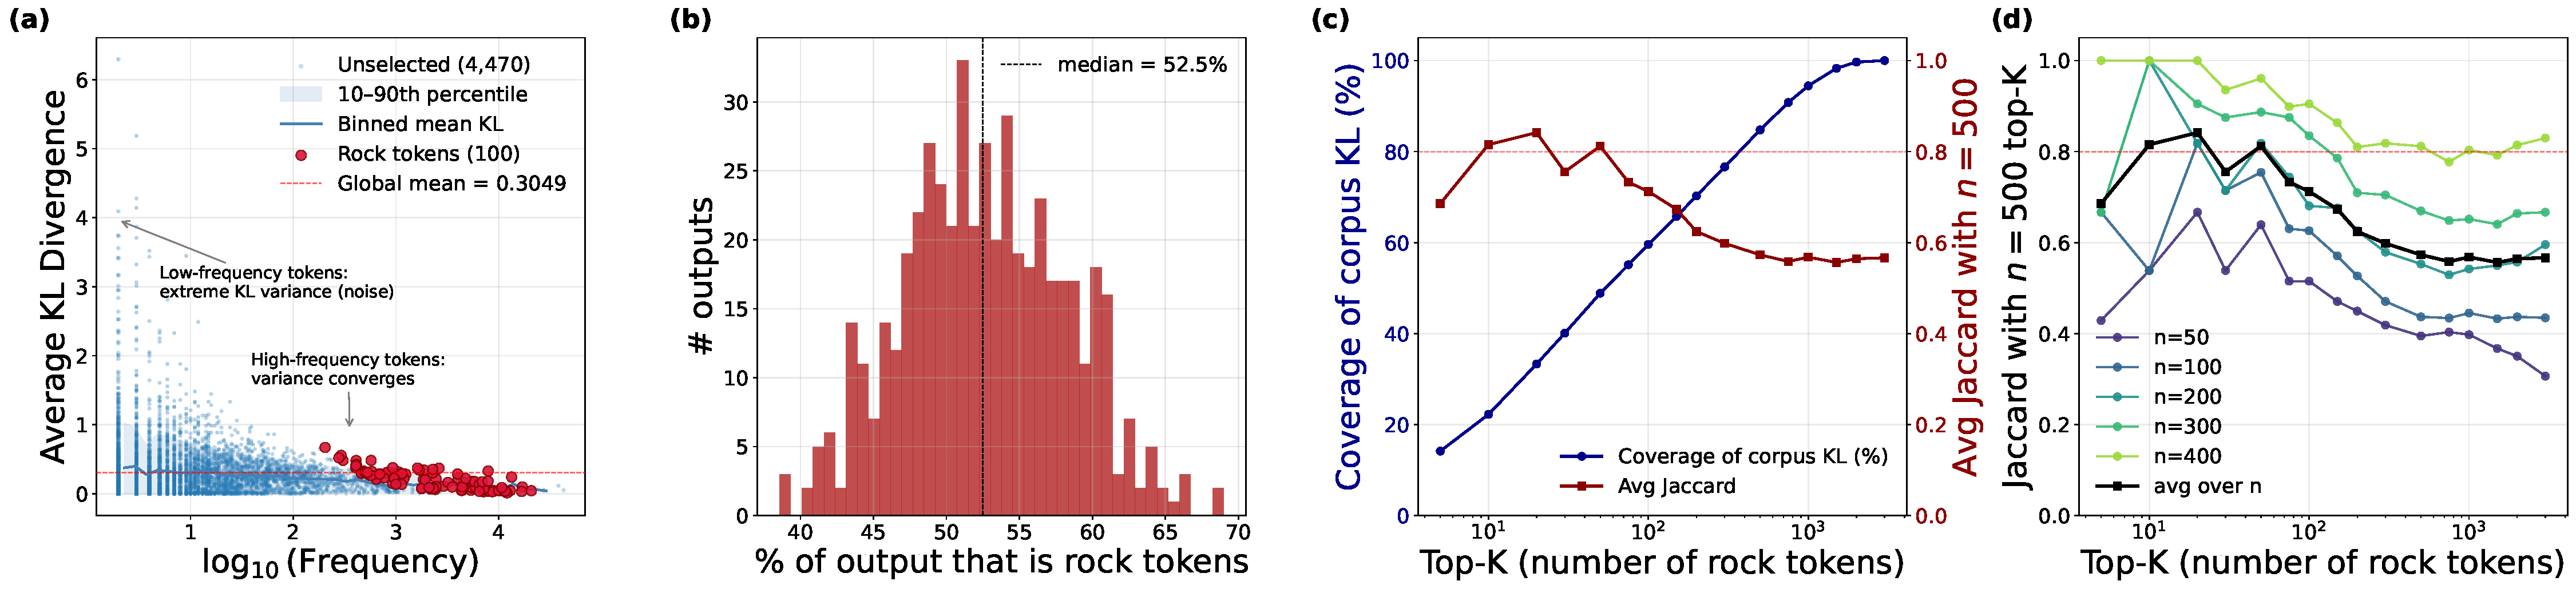
\includegraphics[width=\linewidth]{Figures/Section4/paper_figure1_combined.pdf}
  \caption{\textbf{Empirical identification and stability of Rock Tokens.}
  \textbf{(a)} Per-token KL $\widehat\ell_v$ vs.\ frequency on $N{=}500$
  MATH-500 trajectories: rare tokens are noise-dominated, while the Rock
  Score $R(v)$ isolates true Rock Tokens (red) at the upper edge of stable
  frequency bands. \textbf{(b)} Per-sequence Rock-Token density
  (median $52.5\%$). \textbf{(c)} Cumulative loss coverage (blue) and
  selection stability (red) vs.\ cutoff $K$; $K{=}100$ balances
  reproducibility with $\approx 60\%$ coverage of the distillation burden.
  \textbf{(d)} Jaccard ranking robustness across sample sizes
  $n\in[50,400]$: the top-$100$ selection is stable, larger cutoffs degrade.}

  % \caption{\textbf{Empirical identification and stability of Rock Tokens.} \textbf{(a)} Average KL Divergence ($\widehat\ell_v$) vs. token frequency ($N{=}500$ MATH-500 trajectories). Raw KL exhibits extreme small-sample variance for rare tokens. The Rock Score $R(v)$ bypasses this noise, isolating true Rock Tokens (red dots) at the upper edge of stable frequency bands. \textbf{(b)} Distribution of the percentage of Rock Tokens across generated outputs, indicating a median density of 52.5\% per sequence.\textbf{(c)} Cumulative loss coverage (blue) vs. selection stability (red) across cutoff sizes $K$. The $K{=}100$ boundary optimally balances high reproducibility with $\approx 60\%$ coverage of the total distillation burden. \textbf{(d)} Ranking robustness (Jaccard index) across sample sizes ($n{=}50$--$400$). The Top-100 selection remains highly stable before degrading at noisier cutoffs.}
  \label{fig:rock-id}
\end{figure}













\subsection{Token-Level Loss in On-Policy Distillation}
\label{sec:opd_loss}

On-policy distillation (OPD) optimizes a student policy $\pi_\theta$ by matching a teacher policy $\pi_T$ on trajectories sampled from the student's own distribution. The objective minimizes the per-token reverse KL divergence:
\begin{equation}
\mathcal{L}_{\mathrm{OPD}}(\theta) = \mathbb{E}_{x_{1:T} \sim \pi_\theta} \left[ \sum_{t=1}^{T} D_{\mathrm{KL}} \left( \pi_\theta(\cdot | x_{<t}) \| \pi_T(\cdot | x_{<t}) \right) \right].
\end{equation}
The loss at position $t$ is $\ell_t = \log \pi_\theta(x_t | x_{<t}) - \log \pi_T(x_t | x_{<t})$, measuring the student-teacher mismatch~\cite{fu2026revisiting}. Ideally, as the student aligns with the teacher, the magnitude of $\ell_t$ should systematically diminish across the vocabulary, leading to an optimization plateau where corrective signals eventually vanish.

\subsection{Defining and Detecting Rock Tokens}
\label{sec:rock_tokens}

Contrary to the expected convergence, we observe a subset of tokens that persistently exhibit high KL divergence even after training saturation. We term these \textbf{Rock Tokens}. 

At an intuitive level, our detection method isolates these tokens based on their \textit{Total Distillation Burden}—the absolute volume of optimization capacity consumed by a specific vocabulary item across the entire training corpus. Since the loss $\mathcal{L}_{\mathrm{OPD}}$ is an expectation over student trajectories, it admits an exact additive decomposition over token types $v$ in the vocabulary $\mathcal{V}$:
\begin{equation}
\mathcal{L}_{\text{OPD}}(\theta) = \mathbb{E}_{x \sim \pi_\theta} \left[ \sum_{t} \ell_t \right] = \sum_{v \in \mathcal{V}} \underbrace{\text{Freq}(v) \cdot \mathbb{E}[\ell_t \mid x_t = v]}_{R(v)}
\end{equation}

We formally define the \textbf{Rock Score} as $R(v) = \bar{\ell}_v \cdot \mathrm{Freq}(v)$, where $\bar{\ell}_v$ is the empirically estimated mean KL loss of token $v$ at the final checkpoint. The Rock Score $R(v)$ is therefore not an approximation, but the exact contribution of token type $v$ to the total loss that OPD minimizes. Ranking tokens by $R(v)$ is the unique additive ranking that strictly agrees with the OPD objective.

The $\mathrm{Freq}(v)$ factor acts as a natural regularizer: it up-weights tokens whose mean-loss estimate converges quickly under heavy sampling, while heavily discounting rare tokens whose mean is dominated by small-sample variance. Detection via $R(v)$ thus simultaneously aligns with the theoretical training objective while remaining robust to the empirical estimation noise inherent in natural language generation. 

Operationally, $R(v)$ prioritizes tokens that exhibit both a substantial occurrence count and an above-baseline per-token loss. Rare tokens with extreme observed losses receive appropriately low scores because their $\mathrm{Freq}(v)$ weight is minimal. As demonstrated empirically in Figure~\ref{fig:rock-id}, the top-ranked tokens cluster in the mid-to-high frequency range and sit at the upper edge of the loss distribution within their respective frequency bands, successfully filtering out the rare-but-extreme statistical outliers.








\subsection{Empirical Analysis}
\label{sec:rock_empirical}
Rock tokens exhibit persistently high expected KL divergence between student $\pi_\theta$ and teacher $\pi_T$ after on-policy distillation. We estimate this per-token loss $\widehat\ell_v = \widehat{\mathbb{E}}\big[D_{\mathrm{KL}}\!\big(\pi_\theta(\cdot \mid x_{<t}) \;\|\; \pi_T(\cdot \mid x_{<t})\big) \mid x_t = v\big]$ using student rollouts.

\textbf{Setup} The student (Qwen3-4B-Instruct) is on-policy distilled from the teacher (Qwen3-30B-A3B-Instruct) using OpenThoughts. Per-token KL is sampled from OpenThoughts and evaluated on $N{=}500$ MATH-500 problems (full details in Section~\ref{setup}).

\textbf{Observations} Figure~\ref{fig:rock-id} illustrates the distribution and density of the identified Rock Tokens within the student's generated trajectories. Panel (a) displays the absolute count of Rock Tokens per sequence, while Panel (b) normalizes this count as a percentage of the total sequence length. Strikingly, the data reveals that Rock Tokens are highly concentrated, comprising a median of 52.5\% of the total tokens in every generated output.

\begin{takeaway}
\textcolor{tabblue}{\textbf{Take-away}}~ \textbf{The Pervasiveness of Rock Tokens:} Although Rock Tokens represent a tightly constrained subset of the overall vocabulary (e.g., $K=100$), their footprint during generation is massive. Over half of the model's reasoning trajectory consists of these stubborn structural and formatting tokens, demonstrating that the primary locus of student-teacher disagreement occurs consistently throughout the core scaffolding of the output.
\end{takeaway}


\subsection{Determining the Rock Token Cutoff}\label{sec:cutoff_selection}Defining the boundary of the Rock Token set $\mathcal{R}$ requires choosing a cutoff $K$ that balances \textit{selection stability} (reproducibility across samples) against \textit{loss coverage} (fraction of optimization loss captured). A small $K$ yields a stable set but low coverage, while a large $K$ captures more loss but degrades under sampling noise.

Empirical sweeps (Figures 1b and 1c) identify an optimal intersection at $K=100$. This boundary accounts for roughly 60\% of the corpus-level KL divergence while maintaining high stability across subset sizes. We therefore adopt $K=100$ to ensure a mathematically reproducible vocabulary for subsequent analyses. Comprehensive stability metrics and sweeping procedures are detailed in Appendix \ref{app:rock_ratio}.


% \textbf{Results} Figure~\ref{fig:rock-id}(b) plots Jaccard against $K$, with one curve per $n$ and an averaged curve. Average Jaccard exceeds $0.70$ for $K \leq 100$ and decays toward a $\approx 0.57$ floor for $K \geq 150$ — beyond which the additional tokens are no longer reliably reproduced across sub-corpora. Figure~\ref{fig:rock-id}(c) overlays the corresponding coverage curve: at $K = 100$, $\mathcal{R}$ accounts for $\approx 60\%$ of the corpus-level KL while remaining within the stable regime. We therefore set $K = 100$ ($\approx 2.5\%$ of the observed vocabulary) for the remainder of the paper. This choice represents an explicit tradeoff: $K = 50$ would yield modestly higher stability ($J \approx 0.81$) but reduce coverage to $\approx 49\%$.




\begin{figure*}[t]
  \centering
  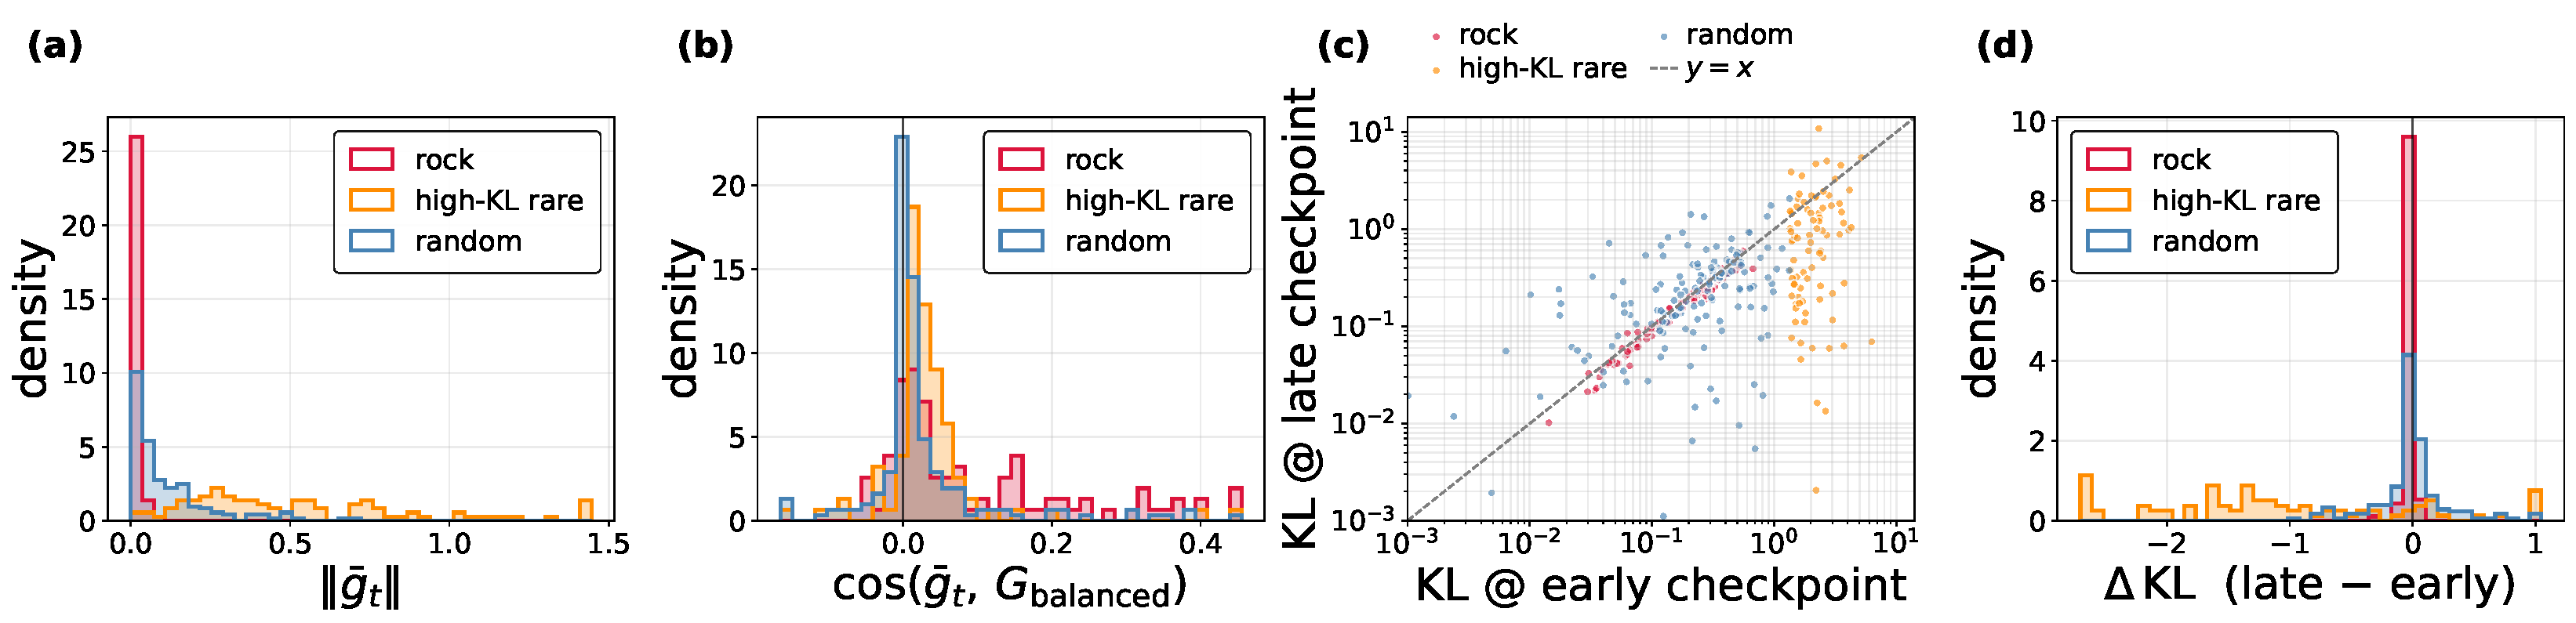
\includegraphics[width=\textwidth]{Figures/Section4/paper_figure2_gradient.pdf}
  \caption{\textbf{Per-token gradient geometry and persistence under
  training.}
  (a) Per-token logit-gradient magnitude $\|\bar{g}_{t}\|$ by group: rocks
  are an order of magnitude smaller than rare high-KL tokens.
  (b) Cosine alignment with the frequency-balanced descent direction
  $G_{\mathrm{balanced}}$: rocks are positively aligned, with a tail
  reaching $\cos > 0.3$.
  (c) Per-token mean KL paired across two training checkpoints (log-log).
  Points below the diagonal indicate KL reduction during further training;
  rocks lie on the diagonal, rare high-KL tokens fall below.
  (d) Distribution of $\Delta\mathrm{KL} = \mathrm{KL}_{\mathrm{late}} -
  \mathrm{KL}_{\mathrm{early}}$ by group: rocks concentrate at
  $\Delta\mathrm{KL} \approx 0$ (persistent); rare high-KL tokens have
  large negative $\Delta\mathrm{KL}$ (learned).}
  \label{fig:gradient}
\end{figure*}


\subsection{Analysis of Rock Tokens}

We decoded the top-$K{=}100$ Rock Tokens into their string forms using the Qwen3 tokenizer. Despite being identified by a purely numerical criterion, the resulting set is functionally coherent: Rock Tokens consistently mark structural or discourse boundaries in mathematical reasoning. 

As detailed in Appendix~\ref{analysis_rock}, four functional clusters dominate $\mathcal{R}$: (1) \textbf{LaTeX and math delimiters}, (2) \textbf{Markdown and whitespace structure}, (3) \textbf{Discourse markers} (e.g., ``So'', ``Wait''), and (4) \textbf{Digits}. In contrast, frequency-matched controls ($\mathcal{S}_{\text{ctrl}}$) predominantly consist of content-bearing tokens (e.g., nouns, verbs) used at non-boundary positions.

\begin{takeaway}
\textcolor{tabblue}{\textbf{Take-away}}~ \textbf{Structure Over Content:} The clustering of $\mathcal{R}$ at boundaries indicates student-teacher divergence centers on \textbf{how to structure} reasoning rather than \textbf{what content} to generate. Rock Tokens are a signature of the on-policy regime, marking where the student systematically resists the teacher's discourse style.
\end{takeaway}



% \subsection{Empirical Observations on Gradient Geometry and Persistence}

% Having established that Rock Tokens primarily comprise syntactic and structural scaffolding, we address \textbf{RQ1: Do Rock Tokens still provide useful learning signals during optimization?} To determine whether their persistent high loss effectively translates into steady directional guidance or merely stagnant optimization noise, we characterize their training dynamics and geometric properties through a comparative analysis against rare high-KL tokens and random tokens (illustrated in Figure~\ref{fig:gradient}). A formal mathematical decomposition of the per-token gradient contributions, alongside complete statistical significance testing, is detailed in Appendix \ref{app:gradient_geometry}. Our findings are summarized as follows:

% \textbf{Low Gradient Magnitude vs. High Frequency (Panel a):} 
%     Rock Tokens are characterized by significantly lower individual logit-gradient magnitudes ($\|\bar{g}_t\|$) compared to standard learnable high-loss tokens. However, because of their massive frequency in the training corpus, this small per-occurrence signal accumulates into a dominant aggregate force on the weight updates.

% \textbf{Alignment with Global Optimization (Panel b):} 
%     Counter-intuitively, the gradient direction of Rock Tokens ($\bar{g}_t$) exhibits a higher cosine similarity with the balanced global gradient ($G_{\text{balanced}}$) than other groups. This suggests that, from the teacher's perspective, Rock Tokens do indeed point toward a "correct" optimization path for the overall objective.

% \textbf{Persistence During Training (Panel c):} 
%     By comparing KL divergence at early versus late checkpoints, we observe that learnable high-KL tokens move significantly below the $y=x$ diagonal, indicating successful optimization. In contrast, Rock Tokens and random tokens cluster closely along the diagonal, demonstrating their resistance to training signals.

% \textbf{Optimization Stagnation (Panel d):} 
%     The distribution of $\Delta \text{KL}$ confirms that Rock Tokens remain largely "untrained," with their change in loss concentrated sharply at zero. While major high-loss tokens show a significant decrease in KL, random tokens exhibit a symmetric, noisy distribution, further highlighting the unique stagnation of Rock Tokens.

% \begin{takeaway}
% \textcolor{tabblue}{\textbf{Take-away}}~ \textbf{The Gradient Paradox:} Rock Tokens \textit{do} provide useful learning signals, generating gradients that are well-aligned with the global optimization target (Panel b). However, they remain stagnant and "untrained" throughout the OPD process (Panel d). This paradox suggests that their persistence is not due to a lack of constructive signal, but rather the student model's internal optimization bias, which stubbornly prioritizes pre-existing structural scaffolding over the teacher's stylistic direction.
% \end{takeaway}




\subsection{Empirical Observations on Gradient Geometry and Persistence}

Having established that Rock Tokens primarily comprise syntactic and structural scaffolding, we address \textbf{RQ1: Do Rock Tokens still provide useful learning signals during optimization?} To determine whether their persistent high loss effectively translates into steady directional guidance or merely stagnant optimization noise, we characterize their training dynamics and geometric properties against rare high-KL tokens and random tokens (illustrated in Figure~\ref{fig:gradient}). 

To formally evaluate this, we analyze the geometry of per-token gradients. For each token type $t$ with $n_{t}$ occurrences, we compute the mean per-occurrence reverse-KL gradient in logit space, $\bar{g}_{t} = \tfrac{1}{n_{t}} \sum_{i} g_{i}$. We then decompose its contribution to the global descent as:
\begin{equation}
\mathrm{contrib}(t) \;=\; n_{t} \,\cdot\, \|\bar{g}_{t}\| \,\cdot\, \cos\bigl(\bar{g}_{t},\, G_{\mathrm{balanced}}\bigr),
\label{eq:contrib}
\end{equation}
where $G_{\mathrm{balanced}} = \sum_{t} \bar{g}_{t}$ is a frequency-balanced reference that grants every token type equal weight, deliberately removing the trivial frequency-weighted dominance of common tokens. This decomposition yields several key insights corresponding to our empirical observations:

\textbf{Low Gradient Magnitude vs. High Frequency (Panel a):} 
Rock tokens are characterized by substantially \emph{smaller} per-occurrence gradient magnitudes than rare high-KL tokens (median $\|\bar{g}_{t}\| \approx 0.016$ versus $\approx 0.54$; Mann-Whitney $p < 10^{-30}$). However, the multiplicative decomposition in Eq.~\ref{eq:contrib} shows that rock dominance arises from the \emph{frequency} factor ($n_t$): because of their massive occurrence rate in the training corpus, this small per-token signal accumulates into a dominant aggregate force on the weight updates.

\textbf{Alignment with Global Optimization (Panel b):} 
Counter-intuitively, the gradient direction of Rock Tokens ($\bar{g}_t$) exhibits non-trivially positive directional alignment with the balanced global gradient $G_{\mathrm{balanced}}$ (median $\cos \approx 0.040$ versus $\approx 0.025$ for high-KL and $\approx 0.006$ for random tokens), with a sub-population reaching $\cos > 0.3$. This means that each rock contributes a small but consistently aligned signal at many positions, whereas rare high-KL tokens contribute large but direction-distinct signals at very few. From the teacher's perspective, Rock Tokens do indeed point toward a ``correct'' optimization path for the overall objective.

\textbf{Persistence During Training (Panel c \& d):} 
To confirm that this directional alignment translates into resistance to further learning, we compare per-token KL between an early and late checkpoint. Rare high-KL tokens experience a substantial reduction in KL (median $2.02 \to 0.85$, $\sim 58\%$; Wilcoxon $p < 10^{-8}$), moving significantly below the $y=x$ diagonal. In contrast, Rock Tokens remain essentially unchanged (median $0.21 \to 0.19$), clustering sharply along the diagonal with the distribution of $\Delta \text{KL}$ concentrated exactly at zero (Panel d). Random control tokens show a symmetric, noisy distribution with no net change.

This optimization stagnation is geometrically consistent with our gradient findings: rare high-KL tokens possess direction-distinct gradients that focused updates can isolate and resolve. Conversely, because rocks contribute highly aligned gradients, their targeted reduction would be indistinguishable from following the global descent. Thus, they receive no separable, token-specific learning signal to overcome their inherent loss.


While our gradient decomposition explains the geometry of this stagnation, the underlying mechanical cause remains open. We hypothesize this paradox is driven by adaptive optimizers under heavy-tailed class imbalance~\cite{kunstner2024heavytailedclassimbalanceadam}. Unlike in pre-training—where Adam beneficially suppresses frequent tokens to avoid overfitting structural noise—On-Policy Distillation often requires updating these exact high-frequency structural tokens to match a teacher's formatting or style. By inflating the second-moment estimates for ubiquitous Rock Tokens, Adam systematically neutralizes their effective learning rate, trapping the student in pre-existing habits despite possessing accurate directional gradients. We leave the formal verification of this optimizer-suppression hypothesis to future work.

\begin{takeaway}
\textcolor{tabblue}{\textbf{Take-away}}~ \textbf{The Gradient Paradox:} Rock Tokens \textit{do} provide useful learning signals, generating gradients that are well-aligned with the global optimization target (Panel b). However, they remain stagnant and "untrained" throughout the OPD process (Panel d). This paradox suggests that their persistence is not due to a lack of constructive signal, but rather the student model's internal optimization bias, which stubbornly prioritizes pre-existing structural scaffolding over the teacher's stylistic direction because the rock-token signal is mathematically inseparable from the global descent direction.
\end{takeaway}








\section{Pillar Tokens: The Scaffolding of Fragile Reasoning}


\subsection{Existence as Necessity: The Functional Value of Rock Tokens}

We have observed that \textbf{Rock Tokens} remain resistant to optimization throughout the entire OPD process. To understand the origin of this resistance, we hypothesize that these tokens serve as the structural ``pillars'' of the model's reasoning process. Under this view, the student model may actively protect these tokens from optimization to prevent its internal reasoning framework from collapsing, even when they conflict with the teacher's distribution. This leads to our \textbf{RQ2: Does Rock Token persistence stem from student path dependency?}


\begin{figure}[h]
  \centering
  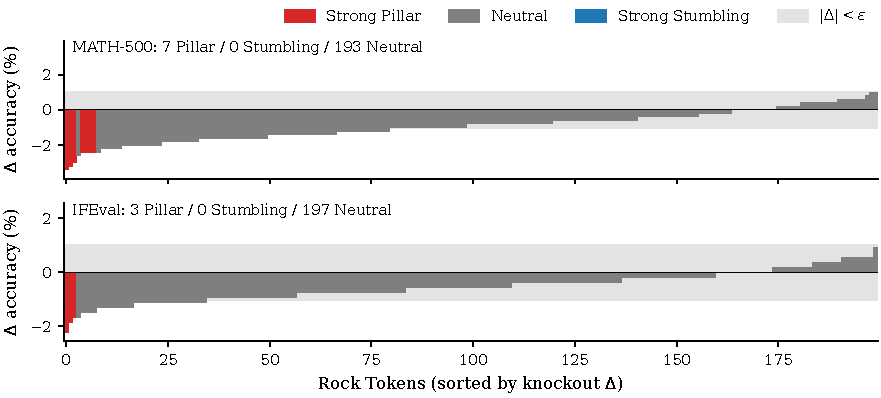
\includegraphics[width=\linewidth]{Figures/Section5/pillar_delta_bar.pdf}
  \caption{\textbf{Knockout effect on the $|\widetilde{\mathcal{R}}|=200$ screened Rock-Token candidates, sorted by $\Delta$.}
  Each bar is a single candidate; height is the accuracy change when its
  logit is masked at decode time. The shaded grey band marks the
  categorization threshold $|\Delta| < \varepsilon = 0.01$. Bars outside the
  band that pass the paired-bootstrap test ($\alpha=0.05$, $10{,}000$
  resamples) are coloured by category (Strong Pillar in red; Strong
  Stumbling in blue). The vast majority of candidates are Neutral on both
  benchmarks; Pillars occupy a short tail and the symmetric Strong-Stumbling
  side is empty --- the visual evidence underlying the sign-asymmetry test
  formalized below.}
  \label{fig:pillar-delta-bar}
\end{figure}
\subsection{Causal Probing via Inference-time Knockout}
\label{sec:knockout_method}

To move beyond distributional metrics and pinpoint the exact functional value of individual tokens, we employ an inference-time \textbf{knockout} procedure. We probe the causal contribution of a token $v$ by observing how its absence affects the model's accuracy on a benchmark $\mathcal{B}$. Specifically, we form a \textit{knockout policy} $\pi_\theta^{\setminus v}$ by forcing the logit of token $v$ to $-\infty$ at every decoding step. We then measure the \textbf{causal delta}:
\begin{equation}
\Delta_{\mathcal{B}}(v) = \mathrm{Acc}_{\mathcal{B}}\bigl(\pi_\theta^{\setminus v}\bigr) - \mathrm{Acc}_{\mathcal{B}}\bigl(\pi_\theta\bigr).
\label{eq:knockout_delta}
\end{equation}
A token $v$ is identified as a \textbf{Strong Pillar} if its removal causes a significant degradation ($\Delta_{\mathcal{B}}(v) \le -0.01$). We screen a pool of $|\widetilde{\mathcal{R}}|=200$ candidates, extending beyond the core $K=100$ set to ensure a wider search for these rare causal effects (see Appendix~\ref{sec:pillar-experiments} for statistical and operational details).

\subsection{Are Rock Tokens Pillars? Findings and Orthogonality}
\label{sec:pillar_findings}

The distribution of $\Delta_{\mathcal{B}}(v)$ in Figure~\ref{fig:pillar-delta-bar} reveals the underlying nature of the Rock Token set. Our investigation yields three primary observations:




\textbf{Pillars are rare but vital:} Only $3.5\%$ of Rock Tokens on MATH-500 and $1.5\%$ on IFEval qualify as Strong Pillars. While most high-KL tokens are neutral residuals, a small subset is absolutely indispensable for the model's reasoning trajectory.
\textbf{Directional Asymmetry:} The complete absence of Strong Stumbling Blocks suggests that the student's "stubborn" deviations from the teacher are rarely detrimental to its own logic; they are either necessary anchors or harmless stylistic preferences.
\textbf{Orthogonality to Traditional Metrics:} 
To examine if Pillarhood can be predicted by standard signals, we analyzed the correlation between $\Delta_{\mathcal{B}}(v)$ and several distributional metrics, including student/teacher entropy, log-frequency, and residual KL. 
Crucially, none of these predictors exhibit a significant correlation with a token's causal importance ($|r| < 0.07$, see Appendix~\ref{sec:pillar-vs-forking} for full analysis and scatter plots). 
This demonstrates that Pillarhood is a property orthogonal to existing importance taxonomies~\cite{tip2026}, suggesting that importance schemes keyed to loss or entropy signals risk suppressing the very tokens the student model cannot reason without.

\begin{takeaway}
\textcolor{tabblue}{\textbf{Take-away}}~
\textbf{The Concentration of Necessity.} 
While Rock Tokens as a population are indispensable for training stability, their causal necessity at inference is highly concentrated: only a tiny fraction ($1.5\%$--$3.5\%$) act as true \textbf{Pillars}. 
This refutes the hypothesis that the student relies on the \textit{entire} high-loss set to maintain reasoning; instead, the model appears to protect a wide "buffer zone" of persistent residuals to ensure a few critical, semantic anchors remain intact.
\end{takeaway}


\section{The genuine contribution of Rock Tokens} 
\label{sec:rq3}



% Early Allies, Late Divergence
% From Allies to Antagonists: The Divergent Trajectory of Gradient Evolution
% Aligned Effort, Diminishing Impact
% 

\begin{wrapfigure}[11]{r}{0.47\columnwidth}
    \vspace{-1.2em}
    \centering
    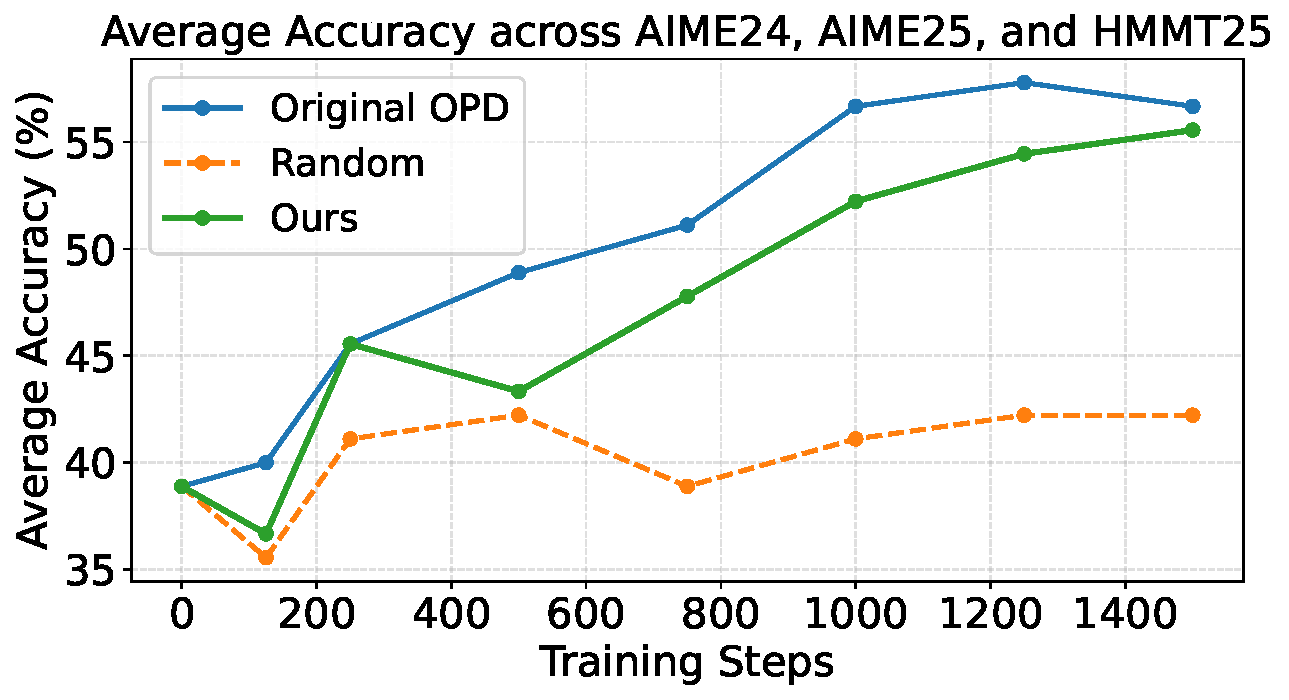
\includegraphics[width=0.45\columnwidth]{Figures/opd_random_vs_ours_avg.pdf}
    \vspace{-0.8em}
    \caption{
    Average accuracy across AIME24, AIME25, and HMMT25 during OPD training. Each 200 training steps correspond to 8,000 prompts, with 4 rollouts per prompt.
    }
    \label{fig:opd_random_vs_ours}
    \vspace{-1.2em}
\end{wrapfigure}
\leavevmode\par
\noindent


\subsection{RQ3: What is the genuine functional contribution of Rock Tokens to model training?}

The functional redundancy of Rock Tokens at inference prompts a critical question: do their persistent high-loss signals provide essential constraints, or are they merely \textbf{optimization noise}? We consider two competing hypotheses: (1) \textbf{Late-stage Saturation}, where these tokens act as early alignment drivers but become unproductive "Stumbling Blocks" as the model reaches structural limits; or (2) \textbf{Inherent Inutility}, where they represent superficial stylistic gaps with no reasoning value from the outset. 

To adjudicate between these views, we employ a \textbf{selective distillation strategy} by freezing the gradients of Rock Tokens. By comparing training trajectories with and without these signals, we aim to determine whether these persistent residuals are indispensable functional anchors or a detrimental optimization burden that consumes gradient bandwidth without yielding performance gains.




\subsection{Selective Distillation via Token-Level Reweighting}
\label{Preliminaries:Stumbling Tokens and Token-Level Reweighting}

To evaluate the functional necessity of these persistent residuals, we introduce a token-level reweighting mechanism to the OPD objective:
\begin{equation}
\mathcal{L}_{\text{weighted}} = \mathbb{E}_{x \sim \pi_\theta} \sum_{t=1}^{T} w(x_t) \cdot \ell_t, \quad \text{where } 
w(v) = \begin{cases} \lambda, & v \in \mathcal{R} \\ 1, & v \notin \mathcal{R} \end{cases}
\end{equation}
Here, $\mathcal{R}$ is the Persistence Set defined in Section~\ref{sec:rock_tokens}, and $\lambda \in [0, 1]$ serves as a scaling factor to modulate optimization pressure. This formulation allows us to test whether the gradient bandwidth consumed by tokens with high Rock Scores $R(v)$ is productive for learning or merely an optimization burden.

Our core experimental design employs three regimes by manipulating $\lambda$. The \textbf{Baseline OPD} ($\lambda=1$) follows standard distillation without intervention. \textbf{Rock-Freeze (Our Method)}: Based on the identified set $\mathcal{R}$, we adopt a radical "Just Not Train" approach by setting $\mathbf{\lambda = 0}$. This strategy effectively \textbf{masks the gradients} of all $v \in \mathcal{R}$, allowing us to determine if these tokens are indispensable functional anchors or simply unproductive residuals that can be bypassed to save computational budget. Finally, the \textbf{Freq-Matched Freeze (Random)} applies the same $\mathbf{\lambda=0}$ strategy to a randomly sampled set $\mathcal{S}$ that strictly matches the \textbf{token frequency distribution} of $\mathcal{R}$. By comparing these three settings, we can decouple the impact of structural Rock Tokens from stochastic noise and frequency-related artifacts.




\subsection{Impact of Rock Tokens on Reasoning Performance}

Figure~\ref{fig:opd_random_vs_ours} illustrates the performance trajectories across AIME24, AIME25, and HMMT25 under different intervention regimes. Our analysis reveals three key findings. First, while Rock Tokens exhibit persistent high loss, they are not merely "noise traps"; their inclusion provides essential gradients that anchor the optimization process, as evidenced by the performance gap between the \textit{Original OPD} and \textit{Ours}. Second, while reducing total gradient signals is generally detrimental—shown by the severe degradation in the \textit{Random} baseline—selectively down-weighting Rock Tokens is significantly safer, maintaining a much higher accuracy ceiling. Third, in our setup, Rock Tokens account for approximately 50\% of the total output tokens; by mitigating the optimization pressure on these residuals, our empirical results demonstrate a 1.7$\times$ increase in overall training wall-clock speed without substantial loss in reasoning integrity.


\begin{takeaway}
\textcolor{tabblue}{\textbf{Take-away}}~
\textbf{The Efficiency-Performance Frontier:} While Rock Tokens provide necessary structural gradients, they exhibit significantly diminishing marginal utility. Our results demonstrate that applying a freeze-weighting to these 30\% high-cost tokens yields a \textbf{1.7$\times$ wall-clock speedup} with minimal impact on reasoning integrity. This confirms that while Rock Tokens are not entirely disposable, \textbf{non-uniform gradient allocation} can effectively bypass computational redundancy in on-policy alignment.
\end{takeaway}

\section{Experiment Setups}
\label{setup}
\subsection{Off-policy and On-policy Distillation}
\label{sec:training_setup}

We implement a two-stage distillation pipeline via the \textbf{KDFlow} framework~\cite{zhang2026kdflow} to transfer knowledge from a teacher, \textbf{Qwen3-30B-A3B-Instruct-2507} (MoE, 3B active), to a student, \textbf{Qwen3-4B-Instruct-2507}~\cite{qwen3technicalreport}, with thinking mode disabled for both. 
\textbf{Stage 1 (Off-Policy):} To achieve initial \textit{all-vocabulary alignment}, the student is trained for one epoch on 20k teacher-generated solutions from \textbf{OpenThoughts3}~\cite{guha2025openthoughts} using a forward KL objective ($\text{kd\_ratio}=0.5$) with cross-entropy. 
\textbf{Stage 2 (On-Policy):} Starting from the Stage 1 checkpoint, the student samples 4 rollouts each prompt from a separate 10k prompts as a checkpoint, (7 checkpoints in total)  and is trained for one epoch on its own trajectories using pure reverse KL ($\text{kd\_ratio}=1.0$). 
Unless specified, all other hyperparameters follow KDFlow defaults; see Appendix~\ref{app:training_details} for full implementation details.
\subsection{Evaluation}
We employ the \textsc{lm-evaluation-harness} framework \cite{eval-harness} for standardized assessment across all benchmarks in a zero-shot setting. To ensure statistical robustness, we report the \textbf{Pass@1} accuracy averaged over five independent runs, accounting for variance in decoding.

Our evaluation suite focuses on challenging competitive mathematics, comprising \textbf{AIME 24}, \textbf{AIME 25}, and \textbf{HMMT 25-Feb} from MathArena~\cite{dekoninck2026matharena}. Each benchmark contains 30 problems; we report the aggregated average score across these 90 tasks as the primary performance metric in our study. We extend our analysis to MATH-500~\cite{lightman2023letsverifystepstep} and IFEval~\cite{zhou2023instruction} to obtain a robust sample size for token-level statistical evaluation.


\section{Related Works}

\subsection{On-Policy Distillation for LLM Post-Training}

On-policy distillation evolves beyond SFT and RLVR by combining trajectory exploration with dense, token-level guidance~\cite{lu2025onpolicydistillation,fu2025pruningweightstruthsafeguarding}. Recent large-scale systems like DeepSeek-V4~\cite{deepseekv4}, MiMo~\cite{xiao2026mimo}, and Qwen-3~\cite{qwen3technicalreport} demonstrate its efficacy as a post-training stage, while self-distillation studies~\cite{zhao2026self,shenfeld2026self,hubotter2026reinforcement} suggest OPD is a general mechanism for amplifying latent model capabilities rather than mere imitation. However, the success of OPD is often hindered by teacher-student misalignment. While prior research examines this incompatibility through global factors like vocabulary, reasoning style, or model family~\cite{fu2026revisiting,li2026rethinking}, our work focuses on a fine-grained source of stagnation. We investigate \textbf{Rock Tokens}—persistent high-loss positions that resist alignment even after training plateaus—to determine when OPD supervision provides productive signals versus unproductive noise.



\subsection{Token-Level Learning Dynamics in Reasoning Models}

Recent studies demonstrate that reasoning in LLMs is disproportionately supported by critical ``anchor'' tokens, the perturbation of which during inference significantly degrades model performance~\cite{gupta2025llms}. In parallel, RLVR research reveals that training is non-uniform~\cite{yang2025token,cheng2026reasoning,wu2025mitigating}, concentrating optimization on high-entropy "forking tokens" that act as decisive branching points for reasoning gains~\cite{wangbeyond,li2025faedkvinfinitewindowfouriertransform}, and further analysis confirms the overall token distribution drift mainly happens on some sparse but crucial tokens~\cite{meng2026sparse}. Although OPD's dense supervision suggests high-loss tokens drive training, their specific contribution mechanism remains unclear—especially when they persist as \textbf{Rock Tokens}. It is unknown whether these recalcitrant positions are indispensable reasoning pillars or merely unproductive residues. We address this gap by systematically analyzing their gradient dynamics and training effects to determine their true role in the OPD process.



\section{Conclusion}
This paper investigates the role of high-loss tokens in On-Policy Distillation, revealing that while they occupy a dominant position in the loss landscape, they are not the decisive factor for performance gains. Our analysis identifies a distinct category of persistent tokens, termed \textbf{Rock Tokens}, despite their significant gradient magnitude and apparent "effort" during optimization, Rock Tokens fail to provide constructive guidance for the model's reasoning capabilities. Notably, our intervention experiments demonstrate that applying a freeze-weighting to these tokens—thereby deprioritizing them during the optimization update—results in negligible impact on downstream performance while achieving a 1.7$\times$ increase in training wall-clock speed. These findings challenge the conventional wisdom that aligning every high-loss token is indispensable for learning. Instead, we advocate for a more resource-efficient, token-selective approach that bypasses the computational redundancy of low-utility tokens to optimize the efficiency-performance frontier in on-policy alignment.







{
\small
\bibliographystyle{abbrvnat} 
\bibliography{ref_raw}
}

\medskip




%%%%%%%%%%%%%%%%%%%%%%%%%%%%%%%%%%%%%%%%%%%%%%%%%%%%%%%%%%%%

\appendix

\section{Limitations}
First, our empirical evaluations rely predominantly on competitive mathematical reasoning; the functional role of Rock Tokens may differ in open-ended generation or coding tasks where structural boundaries are less rigid. Second, our experimental setup utilizes a specific 30B-to-4B distillation pairing, leaving the persistence and geometry of these tokens across different architectural families or vastly larger scales an open question. Finally, to isolate the functional impact of Stumbling Blocks, our mitigation strategy employs a strict binary gradient-freeze mask. While effective for demonstrating causal necessity, this approach is a blunt instrument; future work should explore dynamic reweighting schemes or soft-penalties that gracefully adapt to token-level loss trajectories throughout the optimization process.
\subsection{Ethics Discussion and Risk Assessment}

This work studies model distillation and training dynamics, and does not introduce a deployed system, human-subject data, or sensitive personal data. Its direct societal risks are therefore limited. However, because improvements in language model training may be used in both beneficial and harmful downstream applications, we acknowledge potential dual-use risks, including misuse for generating low-quality or misleading content.

We mitigate these risks by limiting the paper to research analysis and experimental evaluation. Any released code, models, or processed artifacts will be accompanied by appropriate documentation, intended-use information, and license details. All pretrained models, datasets, and software frameworks used in this work are credited, and their licenses and terms of use are respected.

\section{Analysis on Rock Tokens}
\label{analysis_rock}
 We decode the top-$K{=}100$ rock tokens and their frequency-matched controls $\mathcal{S}_{\text{ctrl}}$ into their string forms using the public Qwen3 tokenizer. Despite being identified by a purely numerical criterion ($R(v)$), the resulting set is functionally coherent: rock tokens fall into a small number of identifiable categories, all of which mark structural or discourse boundaries in mathematical reasoning output.

Four functional clusters dominate $\mathcal{R}$.
\begin{enumerate}
\item \textbf{LaTeX and math delimiters} — \$', \verb|\\|, \verb|$$|, \verb|=|, \verb|^|, \verb|{|, \verb|}|, \verb|frac|, \verb|(|, \verb|)|. These mark transitions into and out of math mode and operate at the syntactic boundary between prose and formula.   \item \textbf{Markdown and whitespace structure} — **', \textbackslash n', \textbackslash n\textbackslash n', :\textbackslash n\textbackslash n', ---\textbackslash n\textbackslash n', \#\#\#'. These delimit logical units (paragraphs, section headers, bold spans).   \item \textbf{Discourse markers at sentence-initial position} — So', Let', We', But', Now', Wait', Then', Since', This'. These open new reasoning steps and signal turns in the chain of thought.
\item \textbf{Digits} — every digit 0' through 9' appears in $\mathcal{R}$, each with frequency in the thousands and a non-trivial mean per-token KL. These are tokens that punctuate quantitative statements.
\end{enumerate}

Contrast with the frequency-matched control set. The control set $\mathcal{S}_{\text{ctrl}}$, sampled at the same frequency distribution, is qualitatively different: it consists predominantly of content-bearing tokens used at non-boundary positions — common nouns and verbs of mathematical discourse (e.g.\ triangle', equation', region', expression', must', find', check'), prepositions and conjunctions used mid-clause (as', between', first', right'), and single-letter variable tokens (a', b', i', f', y'). The frequency-matching procedure thus isolates the relevant axis: rocks and controls share the quantity of supervision they receive during OPD, but differ sharply in their syntactic role.

\textbf{Interpretation} The clustering of $\mathcal{R}$ at structural boundaries indicates that the residual student–teacher divergence after on-policy distillation is concentrated at the points where the model decides \emph{how to structure} its reasoning output, rather than \emph{what content} to emit. Decisions like open math mode'', begin a new paragraph'', insert a section header'', or start a new reasoning step with So' versus Then','' are precisely the positions where the OPD loss persists, even after extensive distillation. This observation suggests that rock tokens are not arbitrary statistical outliers but a consistent signature of the on-policy distillation regime: they identify the structural/discourse decisions that the student systematically fails to align with the teacher.
\section{Training and Evaluation Details}
\label{app:training_details}
\subsection{off policy and on policy training}

\paragraph{Training Details.} We distill from Qwen3-30B-A3B-Instruct-2507, a Mixture-of-Experts teacher with $\sim$30B total and $\sim$3B active parameters, into Qwen3-4B-Instruct-2507 as the student, using the KDFlow framework. Both models are run with thinking mode disabled (\texttt{enable\_thinking=False}). Training proceeds in two stages on a single node of $4\times$ H100 (80\,GB) GPUs with FSDP2, bf16, and gradient checkpointing.
  
\paragraph{Stage 1 -- Off-policy KD.} We first sample 20k teacher responses on math prompts drawn from OpenThoughts3 ($\text{temperature}=0.6$, $\text{top\_p}=0.95$, $\text{max\_new\_tokens}=16384$, $\text{TP}=2$ on $2\times$ H100). The student is then trained on these (prompt, teacher-response) pairs with a per-token KL distillation loss combined with cross-entropy at $\text{kd\_ratio}=0.5$ (vanilla KD, forward KL). We use AdamW with learning rate $2\times10^{-5}$, $5\%$ linear warmup, global batch size $128$ (micro-batch $1$), max sequence length $16384$, sample packing, and ring attention of size $2$, for $1$ epoch.

\paragraph{Stage 2 -- On-policy KD.} Initialized from the Stage-1 checkpoint, the student generates $4$ rollouts per prompt ($\text{temperature}=1.0$, $\text{top\_p}=1.0$, $\text{generate\_max\_len}=8000$, $\text{prompt\_max\_len}=800$) on a separate 10k-prompt slice (positions 20k--30k of the same source), and is distilled toward the teacher's token distributions on those rollouts. We use vanilla KD with reverse KL at $\text{kd\_ratio}=1.0$ (pure distillation, no CE), learning rate $2\times10^{-6}$, $5\%$ linear warmup, gradient clipping at $1.0$, global batch size $4$ (micro-batch $1$), and $1$ epoch. The rollout engine uses $1$ engine with $\text{TP}=2$ and the teacher uses $\text{TP}=4$; both engines share GPUs with the trainer via offload-to-CPU sleep/wakeup (\texttt{teacher\_enable\_sleep=True}, \texttt{rollout\_enable\_sleep=True}.

\paragraph{Defaults.} All other hyperparameters are KDFlow defaults; we did not tune optimizer betas, weight decay, dropout, or KD temperature (kept at $1.0$).


\section{Pillar Correlation and Multiple-Testing Analysis}
\subsection{Pillar Correlation Analysis}
\label{app:pillar_correlations}

Table~\ref{tab:pillar-correlations} reports the full set of Pearson correlations between the inference-time knockout effect $\Delta_{\mathcal{B}}(v)$ (Eq.~\ref{eq:pillar-delta}) and nine candidate token-level predictors, measured over the $|\widetilde{\mathcal{R}}|=200$ screened Rock-Token candidates of \S\ref{sec:pillar-experiments} and reported separately for MATH-500 and IFEval. The figure in the main text (Figure~\ref{fig:pillar-vs-predictors}) visualizes a representative subset of six of these predictors on MATH-500; this table is the complete record, including IFEval and the three loss-based features (pre-/post-OPD KL and KL improvement). Across all eighteen $(predictor, benchmark)$ pairs, no correlation reaches $|r| > 0.075$ and no $p$-value falls below $0.30$. The largest observed magnitude on either benchmark is the IFEval correlation with KL improvement ($r{=}+0.071$, $p{=}0.32$), which is well within the noise band expected at $n{=}200$. We therefore cannot reject the null hypothesis $r=0$ for any predictor on either benchmark, supporting the claim in \S\ref{sec:pillar-vs-forking} that Pillarhood is statistically orthogonal to the entropy-, frequency-, and divergence-based importance signals used by prior work~\cite{wangbeyond,tip2026,yang2025token,wu2025mitigating}.

\begin{table}[h]
\centering
\caption{Pearson correlation between the per-token knockout effect $\Delta_{\mathcal{B}}(v)$ and nine candidate predictors over the $|\widetilde{\mathcal{R}}|=200$ screened Rock-Token candidates, reported for MATH-500 and IFEval. $p$-values are two-sided. No correlation reaches $|r|>0.075$ on either benchmark; no $p$-value falls below $0.30$.}
\label{tab:pillar-correlations}
\small
\begin{tabular}{lcccc}
\toprule
\textbf{Predictor} & \multicolumn{2}{c}{\textbf{MATH-500}} & \multicolumn{2}{c}{\textbf{IFEval}} \\
\cmidrule(lr){2-3}\cmidrule(lr){4-5}
 & $r$ & $p$ & $r$ & $p$ \\
\midrule
Frequency                  & $+0.015$ & $0.832$ & $+0.030$ & $0.677$ \\
Rock count                 & $+0.013$ & $0.855$ & $+0.023$ & $0.751$ \\
Rock rate                  & $-0.022$ & $0.760$ & $-0.047$ & $0.512$ \\
Pre-OPD KL                 & $-0.017$ & $0.808$ & $-0.015$ & $0.833$ \\
Post-OPD KL                & $+0.010$ & $0.883$ & $-0.048$ & $0.503$ \\
KL improvement             & $-0.062$ & $0.386$ & $+0.071$ & $0.320$ \\
Teacher entropy            & $+0.063$ & $0.378$ & $-0.036$ & $0.611$ \\
Pre-OPD student entropy    & $+0.059$ & $0.406$ & $-0.069$ & $0.331$ \\
Post-OPD student entropy   & $+0.056$ & $0.432$ & $-0.037$ & $0.604$ \\
\bottomrule
\end{tabular}
\end{table}

\subsection{Multiple-Testing Analysis for the Per-Token Pillar Criterion}
\label{app:pillar_multiple_testing}

The per-token Pillar criterion of \S\ref{sec:pillar-identification} applies a paired bootstrap test at $\alpha=0.05$ independently to each of the $|\widetilde{\mathcal{R}}|=200$ screened Rock-Token candidates, conjoined with the effect-size filter $|\Delta_\mathcal{B}(v)|\ge\varepsilon$ ($\varepsilon=0.01$). Because $\varepsilon$ is approximately at the per-token sampling-error scale, the conjunction does not appreciably reduce the per-test Type-I rate, and $200\!\times\!0.05 = 10$ rejections are expected under the global null. We report below how the per-token identifications behave under standard family-wise and false-discovery corrections, and the global sign-asymmetry test on which the population-level claim of \S\ref{sec:pillar-experiments} rests.

\paragraph{Per-token corrections.} Bonferroni control of the family-wise error at $\alpha=0.05$ requires $p<\alpha/200=2.5\times 10^{-4}$. The smallest observed $p$-values are $0.0038$ (MATH-500, ``\,certain'') and $0.0016$ (IFEval, ``-like''); neither passes Bonferroni, and consequently no token does. Benjamini--Hochberg control of the false discovery rate at $q\in\{0.05, 0.10, 0.20\}$ likewise produces zero rejections on either benchmark: the BH cutoff $p_{(k)}\le (k/n)\,q$ is not crossed even for the smallest-$p$ token, because $1/200 \times 0.20 = 10^{-3} < 0.0016$. The per-token Pillar identifications are therefore \emph{exploratory candidates}, not confirmatory rejections in the multiple-testing sense.



\paragraph{Global sign-asymmetry test.} The exploratory candidates do, however, exhibit a non-trivial structural property: the sign of the significant rejection is consistent across benchmarks. Of the seven MATH-500 candidates, all seven satisfy $\Delta_{\mathrm{MATH500}}(v)<0$ (Pillar direction); of the three IFEval candidates, all three satisfy $\Delta_{\mathrm{IFEval}}(v)<0$. Combined, the rejection sign-distribution is $10$ negative, $0$ positive. Under the global null in which every per-token rejection is a chance event, the rejection sign should be Bernoulli$(\nicefrac{1}{2})$, and the probability of observing all $10$ on one side is $2^{-10}\approx 9.8\times 10^{-4}$ (two-sided exact binomial $p = 1.95\times 10^{-3}$). On MATH-500 alone the analogous sign test is $7/0$ with two-sided $p=0.016$; on IFEval alone $3/0$ with $p=0.25$. The combined test is a single global test that does not inflate with the number of tokens screened, and it is the result on which \S\ref{sec:pillar-experiments} relies for the population-level claim that a non-empty subset of Rock Tokens is causally necessary at decode time.

\paragraph{Summary.} The reader is advised to read the per-token Pillar identifications of \S\ref{sec:pillar-experiments} (e.g.\ ``\,certain'', ``\,strategic'', ``\,Initialize'') as the strongest individual candidates from a population-level effect, rather than as $7$ independently-confirmed discoveries. The empirical contribution of this section that survives strict multiple-testing scrutiny is the sign asymmetry, which is incompatible with the multiplicity-noise null at $p\approx 0.002$.

\paragraph{Stable-core robustness check.} The screening pool of \S\ref{sec:pillar-identification} is the top-$K_{\text{screen}}=200$ count-ranked extension of $\mathcal{R}$, while the definitional Rock-Token set fixed by the stability/coverage analysis of \S\ref{ref:recalcitrant_tokens} is the top-$K=100$. The 10 Strong Pillars from the bootstrap distribute as follows over the count-rank index. On MATH-500 (ranks reported on the top-200 list): ``\,certain'' (16), ``\,Initialize'' (93), ``\,strategic'' (99), ``Do'' (109), ``\,programs'' (143), ``\,tech'' (166), ``\,arms'' (185). On IFEval: ``-like'' (35), ``\,tools'' (64), ``\,trade'' (69). Six of the ten lie within the $K=100$ core, including the smallest-$p$ token on each benchmark (``\,certain'' at $p=0.0038$ on MATH-500 and ``-like'' at $p=0.0016$ on IFEval). The remaining four lie in the rank-$109$-to-$185$ regime, which \S\ref{ref:recalcitrant_tokens} flags as below the Jaccard-stability sweet spot; we therefore caution that those four are at greater risk of being corpus-specific. The sign-asymmetry test of the previous paragraph is robust to this concern: restricted to the $K=100$ stable core, it remains $6/0$ negative-versus-positive, with two-sided exact-binomial $p = 2^{-6}\!\times\!2 = 3.1\times 10^{-2}$.








\subsection{Definition and Identification of `Pillar Tokens'}
\label{sec:pillar-identification}

To investigate this, we operationally categorize Rock Tokens based on their causal impact at inference time. \textbf{Pillar Tokens} are defined as those whose removal or perturbation degrades task accuracy, suggesting the model \emph{cannot reason without them}, while the remainder are deemed functionally neutral. 

\emph{\textbf{Intuition.}} The core idea is that if a token is truly load-bearing for reasoning, deleting it from the decoder should break the trajectory; if it only \emph{looks} ``hard'' due to high loss but lacks functional utility, its deletion should change nothing. We operationalize Pillarhood as exactly this causal, inference-time property. Given the post-OPD student $\pi_\theta$ and a candidate $v\in\widetilde{\mathcal{R}}$ (screening pool defined below), we form a knockout policy $\pi_\theta^{\setminus v}$ that sets the logit of $v$ to $-\infty$ at every decoding step and record the accuracy delta on a held-out benchmark $\mathcal{B}$:
\begin{equation}
\Delta_{\mathcal{B}}(v) = \mathrm{Acc}_{\mathcal{B}}\bigl(\pi_\theta^{\setminus v}\bigr) - \mathrm{Acc}_{\mathcal{B}}\bigl(\pi_\theta\bigr).
\label{eq:pillar-delta}
\end{equation}
A candidate $v$ is a \textbf{Strong Pillar} on $\mathcal{B}$ iff (i) $\Delta_\mathcal{B}(v)\le-\varepsilon$ ($\varepsilon=0.01$) and (ii) a paired bootstrap on per-problem indicators ($10{,}000$ resamples, $\alpha=0.05$) rejects $\mathrm{H}_0\!:\!\Delta=0$; symmetric thresholds at $+\varepsilon$ define Strong Stumbling Blocks, and all other candidates are Neutral. Accuracies are estimated by sampling at $T{=}1.0$ and averaging over independent rollouts to keep single-trajectory variance below the $\sim\!2\%$ effect scale.

The screening pool is a strict superset $\widetilde{\mathcal{R}}\supset\mathcal{R}$ of size $K_{\text{screen}}=200$ rather than the definitional $K=100$ set $\mathcal{R}$ of \S\ref{sec:rock_tokens}: $K=100$ is the stability/coverage sweet spot when $\mathcal{R}$ is treated as a vocabulary (qualitative analysis, gradient-zeroing in \S\ref{sec:rq3}), but Pillarhood is a per-token causal property and the bootstrap is a search for individual rare-but-real effects, so we trade selection stability below rank $100$ for a wider candidate pool. As a robustness check (Appendix~\ref{app:pillar_multiple_testing}), $6$ of the $10$ Strong Pillars --- including the strongest on each benchmark, ``\,certain'' on MATH-500 and ``-like'' on IFEval --- lie within the $K=100$ core. We probe the post-OPD student on two complementary benchmarks: MATH-500~\cite{lightman2023letsverifystepstep} for the trained reasoning capability and IFEval~\cite{zhou2023instruction} for instruction-following as an out-of-distribution control.


\subsection{Are Rock Tokens pillar? Experiments and findings}
\label{sec:pillar-experiments}

Table~\ref{tab:pillar-census} reports the full Pillar census from the bootstrap procedure across the $|\widetilde{\mathcal{R}}|=200$ screened candidates. The dominant feature of the per-token $\Delta_\mathcal{B}(v)$ distribution is not the tail but the centre: on both benchmarks the great majority of candidates fall inside the $\varepsilon$-band, indicating no detectable causal effect of their removal (visualization in Fig.~\ref{fig:pillar-delta-bar}, Appendix~\ref{app:pillar_multiple_testing}).

\begin{table}[t]
\centering
\caption{Pillar census over the $|\widetilde{\mathcal{R}}|=200$ screened Rock-Token candidates, by benchmark.}
\label{tab:pillar-census}
\begin{tabular}{lcccc}
\toprule
\textbf{Benchmark} & \textbf{Strong Pillar} & \textbf{Neutral} & \textbf{Strong Stumbling} & \textbf{Baseline acc.} \\
\midrule
MATH-500 & 7 (3.5\%)  & 193 (96.5\%) & 0 (0.0\%) & 0.750 \\
IFEval   & 3 (1.5\%)  & 197 (98.5\%) & 0 (0.0\%) & 0.752 \\
\midrule
\multicolumn{4}{l}{Cross-task agreement: 190 N$|$N, 7 P$|$N, 3 N$|$P, \textbf{0} P$|$P} & \\
\bottomrule
\end{tabular}
\end{table}

\paragraph{Multiple-testing considerations.} At $|\widetilde{\mathcal{R}}|=200$ candidates, $\sim\!10$ false rejections are expected by chance at $\alpha=0.05$, and neither Bonferroni nor Benjamini--Hochberg ($q\le 0.20$) retains any individual token (Appendix~\ref{app:pillar_multiple_testing}). We therefore read the per-token identifications above as exploratory \emph{candidate} Pillars. The population-level claim is carried by the \emph{sign} of the rejections: all $10$ fall on the Pillar (negative-$\Delta$) side and zero on the Stumbling side, a $10{:}0$ split with exact probability $2^{-10}\approx 0.002$ under the multiplicity-noise null --- a single global test that does not inflate with the number of candidates screened.

\medskip

Three observations follow. \textbf{First}, Pillars are rare: $3.5\%$ on MATH-500 and $1.5\%$ on IFEval --- the persistent high-KL criterion of \S\ref{ref:recalcitrant_tokens} over-selects causally relevant tokens by more than an order of magnitude. \textbf{Second}, Pillarhood is task-specific: no token is a Strong Pillar on both benchmarks (P$|$P$=0$ in Table~\ref{tab:pillar-census}), so the role of a token type depends on the task. \textbf{Third}, Strong Pillars are content-bearing tokens at decision points, not the structural delimiters that dominate the surface clustering of $\mathcal{R}$ in \S\ref{ref:recalcitrant_tokens}: MATH-500 examples include ``\,certain'', ``\,strategic'', ``\,Initialize'', ``\,programs'', ``Do''; IFEval includes ``\,tools'', ``\,trade'', ``-like''. The symmetric Strong-Stumbling direction is empty under inference-time knockout, an asymmetry we revisit at training time in \S\ref{sec:rq3}.


\subsection{Does Rock Token follow previous findings on `Forking Tokens'?}
\label{sec:pillar-vs-forking}

\emph{Intuition.} The dominant prior framing casts ``important tokens'' as high-entropy decision points where the policy splits between alternative reasoning continuations: forking tokens in RLVR~\cite{wangbeyond}, and the (entropy~$\cup$~student--teacher-divergence) taxonomy formalized for OPD by TIP~\cite{tip2026} and related token-reweighting work~\cite{yang2025token,wu2025mitigating}. If our Pillars were the inference-time projection of any of these training-time importance criteria, knockout $\Delta_\mathcal{B}(v)$ should be predicted by entropy, by KL, or by some combination thereof.

\begin{figure}[t]
  \centering
  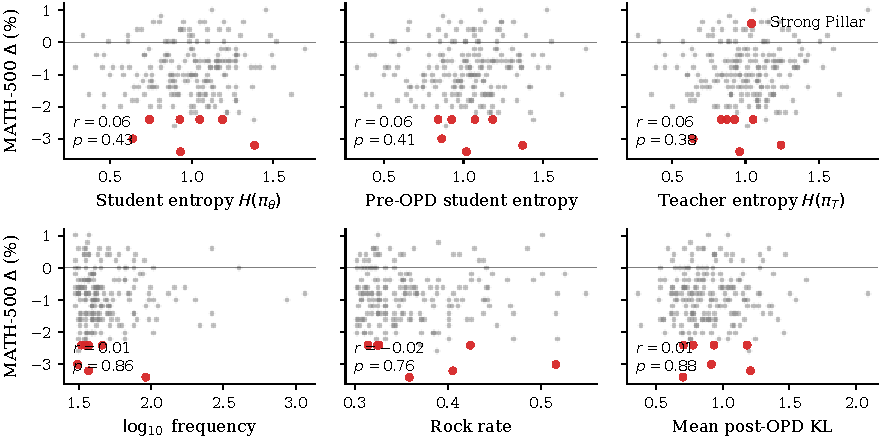
\includegraphics[width=\linewidth]{Figures/Section5/pillar_vs_predictors.pdf}
  \caption{\textbf{Pillarhood is not predicted by entropy, frequency, or
  loss.} MATH-500 knockout $\Delta$ for each of the $|\widetilde{\mathcal{R}}|=200$ screened candidates
  (Strong Pillars in red) plotted against six candidate predictors:
  post- and pre-OPD student entropy, teacher entropy, log-frequency, rock
  rate, and mean post-OPD KL. Annotated $r,p$ are Pearson correlations
  over all 200 candidates. None reach $|r|>0.07$.}
  \label{fig:pillar-vs-predictors}
\end{figure}

\emph{Findings.} Figure~\ref{fig:pillar-vs-predictors} scatters MATH-500 knockout $\Delta_{\mathrm{MATH500}}(v)$ against six candidate predictors --- pre/post-OPD student entropy, teacher entropy, $\log_{10}$ frequency, rock rate, and post-OPD KL --- and \emph{none} reaches $|r|>0.07$; the same conclusion holds on IFEval and on three additional loss-based predictors (Table~\ref{tab:pillar-correlations}, Appendix~\ref{app:pillar_correlations}). Pillars are scattered across the entire entropy range, not concentrated where forking tokens reside, and they are not the tokens with the largest residual KL --- the criterion that $\mathcal{R}$ itself maximizes. Pillarhood is therefore an \emph{orthogonal} cut: a causal, behaviour-defined property that the existing entropy- and divergence-based taxonomies fail to surface, with the immediate methodological corollary that any token-importance scheme keyed to those signals risks suppressing exactly the tokens the student cannot reason without.

\begin{takeaway}
\textcolor{tabblue}{\textbf{Take-away}}~
Pillar Tokens are not Forking Tokens. Their causal role at inference is
uncorrelated with student entropy, teacher entropy, frequency, or
post-OPD KL ($|r| < 0.07$ on MATH-500), placing them outside the
importance taxonomies of prior work~\cite{wangbeyond,tip2026}.
\end{takeaway}



\section{Selection of Ratio}
\label{app:rock_ratio}
Choosing the selection size. The score $R(v)$ provides a ranking; we still need a cutoff $K$ that determines $|\mathcal{R}|$. Two competing criteria bear on this choice. First, $K$ should be small enough that the top-$K$ set is stable — i.e., reproducible across resamplings of the rollout corpus. Second, $K$ should be large enough that $\mathcal{R}$ accounts for a substantial fraction of the corpus-level KL, so that reweighting decisions made on $\mathcal{R}$ have meaningful effect on $\mathcal{L}_{\text{OPD}}$.

\textbf{Procedure} We sweep $K$ jointly with sample size. For each $n \in {50, 100, 200, 300, 400}$, we compute $\widehat R(v)$ from the corresponding sub-corpus and select its top-$K$ tokens; we then measure the Jaccard index of this set against the top-$K$ obtained at $n = 500$. We additionally compute the cumulative coverage $\sum_{v \in \mathcal{R}} \widehat R(v) / \mathcal{L}_{\text{OPD}}^{\text{corpus}}$ at $n = 500$ as $K$ grows.


\textbf{Results} Figure~\ref{fig:rock-id}(b) plots Jaccard against $K$, with one curve per $n$ and an averaged curve. Average Jaccard exceeds $0.70$ for $K \leq 100$ and decays toward a $\approx 0.57$ floor for $K \geq 150$ — beyond which the additional tokens are no longer reliably reproduced across sub-corpora. Figure~\ref{fig:rock-id}(c) overlays the corresponding coverage curve: at $K = 100$, $\mathcal{R}$ accounts for $\approx 60\%$ of the corpus-level KL while remaining within the stable regime. We therefore set $K = 100$ ($\approx 2.5\%$ of the observed vocabulary) as the \emph{definitional} Rock-Token set $\mathcal{R}$ used wherever a stable, reproducible vocabulary is required --- the qualitative cluster analysis below, and the training-time interventions of Section~\ref{sec:rq3}. This choice represents an explicit tradeoff: $K = 50$ would yield modestly higher stability ($J \approx 0.81$) but reduce coverage to $\approx 49\%$. For the per-token causal analysis of Appendix~\ref{sec:pillar-experiments} we instead \emph{screen} a strict superset of size $K_{\text{screen}}=200$: that section's bootstrap is a search for individual rare-but-real Pillars, and the broader candidate pool both increases the chance of detection and lets us probe the regime in which selection stability has decayed below $J\!\approx\!0.6$. The two cutoffs serve different purposes --- the smaller $K$ defines $\mathcal{R}$, the larger one widens the screening window --- and we are explicit in Appendix~\ref{sec:pillar-identification} about which is in force.




%%%%%%%%%%%%%%%%%%%%%%%%%%%%%%%%%%%%%%%%%%%%%%%%%%%%%%%%%%%%

\newpage
\input{checklist.tex}


\end{document}